\documentclass[11pt]{ctexart}
\usepackage{amsmath,amssymb}
\usepackage{graphicx}
\usepackage{enumitem}
\setlist{nosep}
\usepackage{titlesec}
\titlespacing*{\section}{0pt}{7pt}{3pt}
\setlength{\parskip}{3pt}
\usepackage{geometry}
\geometry{a4paper,margin=1.9cm}
\setlength{\parskip}{4pt}

\begin{document}

\begin{center}\Large\bfseries KKT + 二阶判别题 · 考前速查卡\end{center}
\vspace{2pt}
\hrule
\vspace{4pt}

\section*{一、主线（一句话）}

\fbox{\parbox{0.94\textwidth}{\centering\textbf{列 KKT 提名 $\to$ 分内外两支解候选 $\to$ 逐个用临界锥过二阶 $\to$ 单独论证全局}}}

\section*{二、流程}

\begin{enumerate}\setlength{\itemsep}{1pt}
\item 写 $L=f-\sum_i u_i g_i(x)$（本课程口径，\textbf{减号}）；
\item 列 KKT 四条：稳定性 $\nabla_x L=0$；乘子 $u\ge 0$；可行 $g(x)\ge 0$；互补松弛 $u\,g(x)=0$；
\item \textbf{按互补松弛分两支}：
  \begin{itemize}\setlength{\itemsep}{0pt}
  \item 支 A（内点 $g>0$）：$u=0$，解 $\nabla f=0$，回代验证 $g>0$；
  \item 支 B（边界 $g=0$）：边界方程与梯度方程联立。
  \end{itemize}
\item 筛候选：代回 $u\ge0$ 与 $u\,g=0$，$u<0$ 的伪候选扔掉；
\item 逐个过二阶：① 算 $\nabla^2_{xx}L=\nabla^2 f-u\nabla^2 g$；② 写临界锥 $\mathcal C=\{d\ne0\mid \nabla g(x^*)^\top d=0\}$；③ 判 $d^\top\nabla^2_{xx}L\,d$ 在锥上的符号；
\item 全局：$f$ 凸且可行域凸 $\Rightarrow$ 局部即全局；否则（如可行域非凸）找显式下界。
\end{enumerate}

\section*{三、每步要点与易错点}

\begin{center}\footnotesize
\begin{tabular}{p{2.6cm} p{6.4cm} p{6.6cm}}
\hline
\textbf{步骤} & \textbf{动作} & \textbf{易错点} \\
\hline
1.\ 写 $L$ & 口径 $L=f-\sum u_i g_i$ & 写成加号，后面全错 \\
2.\ 列 KKT & 四条默写，尤重互补松弛 & 漏 $u\ge0$ \\
3.\ 分两支 & \textbf{两支都写}；支 A 空手也要写``解得但不满足 $g>0$，舍去'' & 只解边界 $\Rightarrow$ 丢 $u=0$ 候选（全局最小点常在这支） \\
4.\ 筛候选 & 每个点代回四条验证 & 伪候选没扔 \\
5.\ 过二阶 & 减号算 $\nabla^2_{xx}L$；锥内判符号 & ① 减号写加；② 忘了锥、拿全空间判 \\
6.\ 全局 & 凸规划才可说``局部即全局'' & 拿凸规划跳步（可行域非凸时） \\
\hline
\end{tabular}
\end{center}

\section*{四、二阶判读小抄（结论怎么写）}

\begin{itemize}\setlength{\itemsep}{1pt}
\item 锥内 $d^\top\nabla^2_{xx}L\,d>0$ 全成立 $\Rightarrow$ ``二阶充分条件满足 $\Rightarrow$ \textbf{严格局部极小点}''；
\item 锥内存在负值 $\Rightarrow$ ``二阶\textbf{必要}条件被违反 $\Rightarrow$ \textbf{不是局部极小点}''（枪毙路线）；
\item 出现零值 $\Rightarrow$ 二阶不断案，回一阶条件或定义（本题未遇到）。
\end{itemize}

\section*{五、解方程两个技巧}

\begin{itemize}\setlength{\itemsep}{1pt}
\item 梯度方程出现 $x_2=u x_2$ 型（同变量两边）$\Rightarrow$ 必分``$x_2=0$ 或 $u=1$''讨论，这是 KKT 方程组的常规突破口；
\item 边界支：把边界方程代回梯度方程消元，比硬解方程组快。
\end{itemize}

\newpage

\section*{六、应用样例（2026-11-17 练题）}

\textbf{题目：}\quad
$\min\ f(x_1,x_2)=(x_1+1)^2+x_2^2$\quad s.t.\quad $g(x_1,x_2)=x_1^2+x_2^2-1\ge 0$

要求：① 求所有 KKT 点（含乘子）；② 对每个 KKT 点用二阶充分条件判别；③ 指出全局最小点和最小值。

\vspace{2pt}
\textbf{直观图：}\par\vspace{2pt}
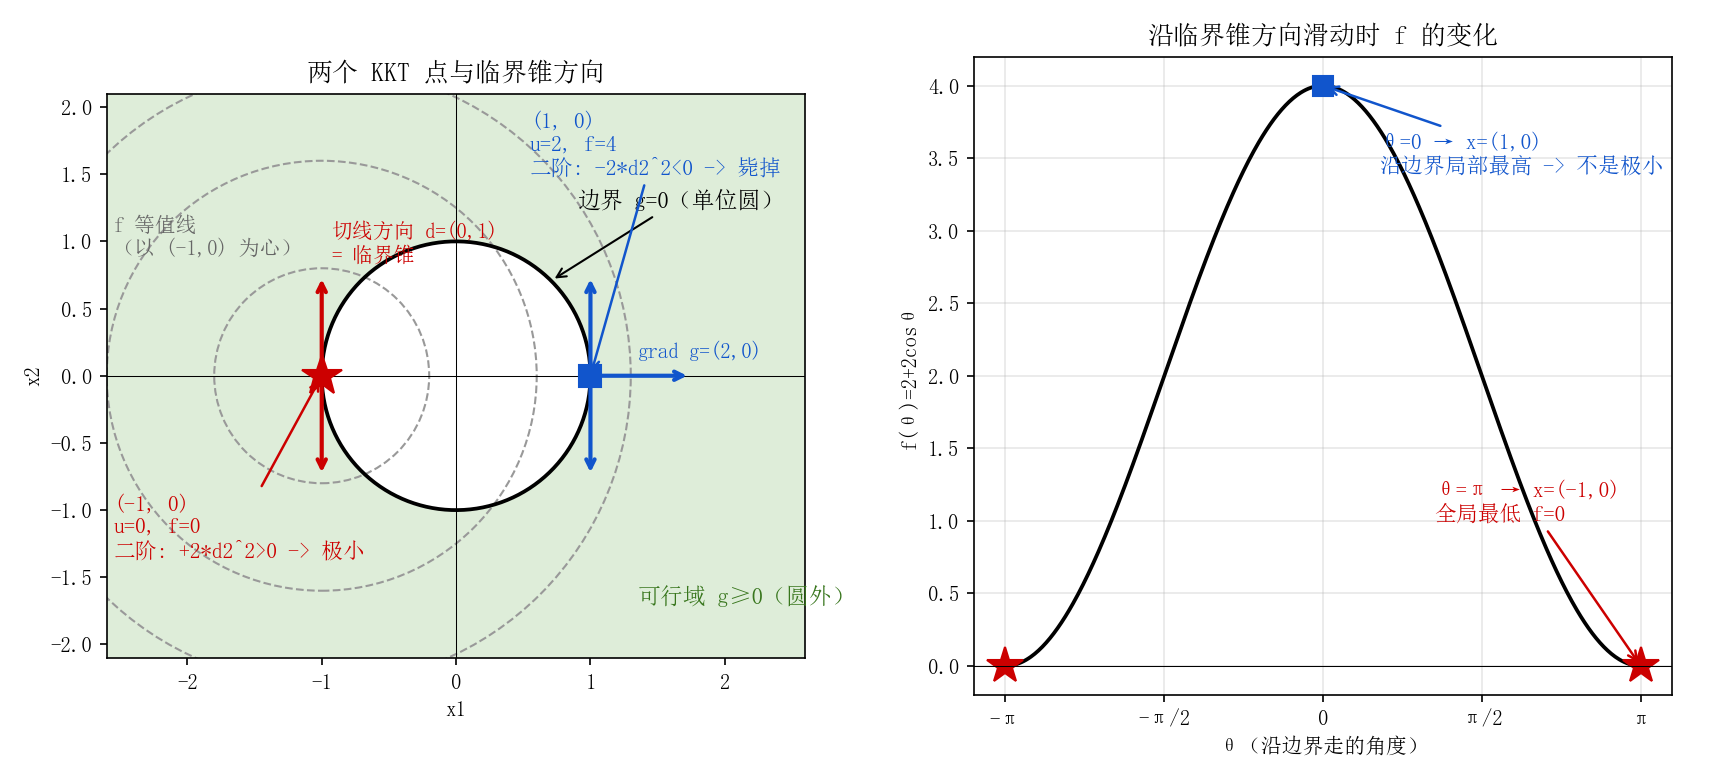
\includegraphics[width=\textwidth]{练习题-KKT二阶-直观图-2026-11-17.png}

\section*{七、答案要点}

\begin{enumerate}\setlength{\itemsep}{1pt}
\item 支 A（$g>0$）：$u=0$，$\nabla f=0$ 解得 $(-1,0)$，但 $g=0$ 在边界，舍去，此支无候选；
\item 支 B（$g=0$）：由 $x_2=ux_2$ 分两种情形（$u=1$ 代入矛盾）$\Rightarrow x_2=0$，$u=\dfrac{x_1+1}{x_1}$，结合 $x_1^2=1$：
  \[ \text{KKT 点：}\ (-1,0)\ (u=0),\qquad (1,0)\ (u=2) \]
\item 二阶：$\nabla^2_{xx}L=2(1-u)I$，临界锥均为 $d_1=0$：
  \begin{itemize}\setlength{\itemsep}{0pt}
  \item $(-1,0)$：$d^\top(2I)d=2d_2^2>0$ $\Rightarrow$ 严格局部极小；
  \item $(1,0)$：$d^\top(-2I)d=-2d_2^2<0$ $\Rightarrow$ 必要条件被违反，不是局部极小。
  \end{itemize}
\item 全局：$f\ge0$ 且 $(-1,0)$ 可行 $\Rightarrow$ $x^*=(-1,0)$，$f^*=0$。
\end{enumerate}

\vspace{4pt}
\hrule
\vspace{3pt}
{\small 完整推导与易错点见《练习题-KKT点判别与二阶充分条件-2026-11-17.pdf》。}

\end{document}
